\subsection{Mapping}
\label{sec:models/kf/mapping}
In the mapping problem, we assume we don't have the knowledge of the map $\vec M$ (described in subsection \ref{subsec:models/kf/localisation}), but know the vehicle states $\vec x_1, \dotsc, \vec x_T$ exactly. We want to figure out $\vec M$. The graphical model is as follows
\begin{figure}[!htb]
\centering
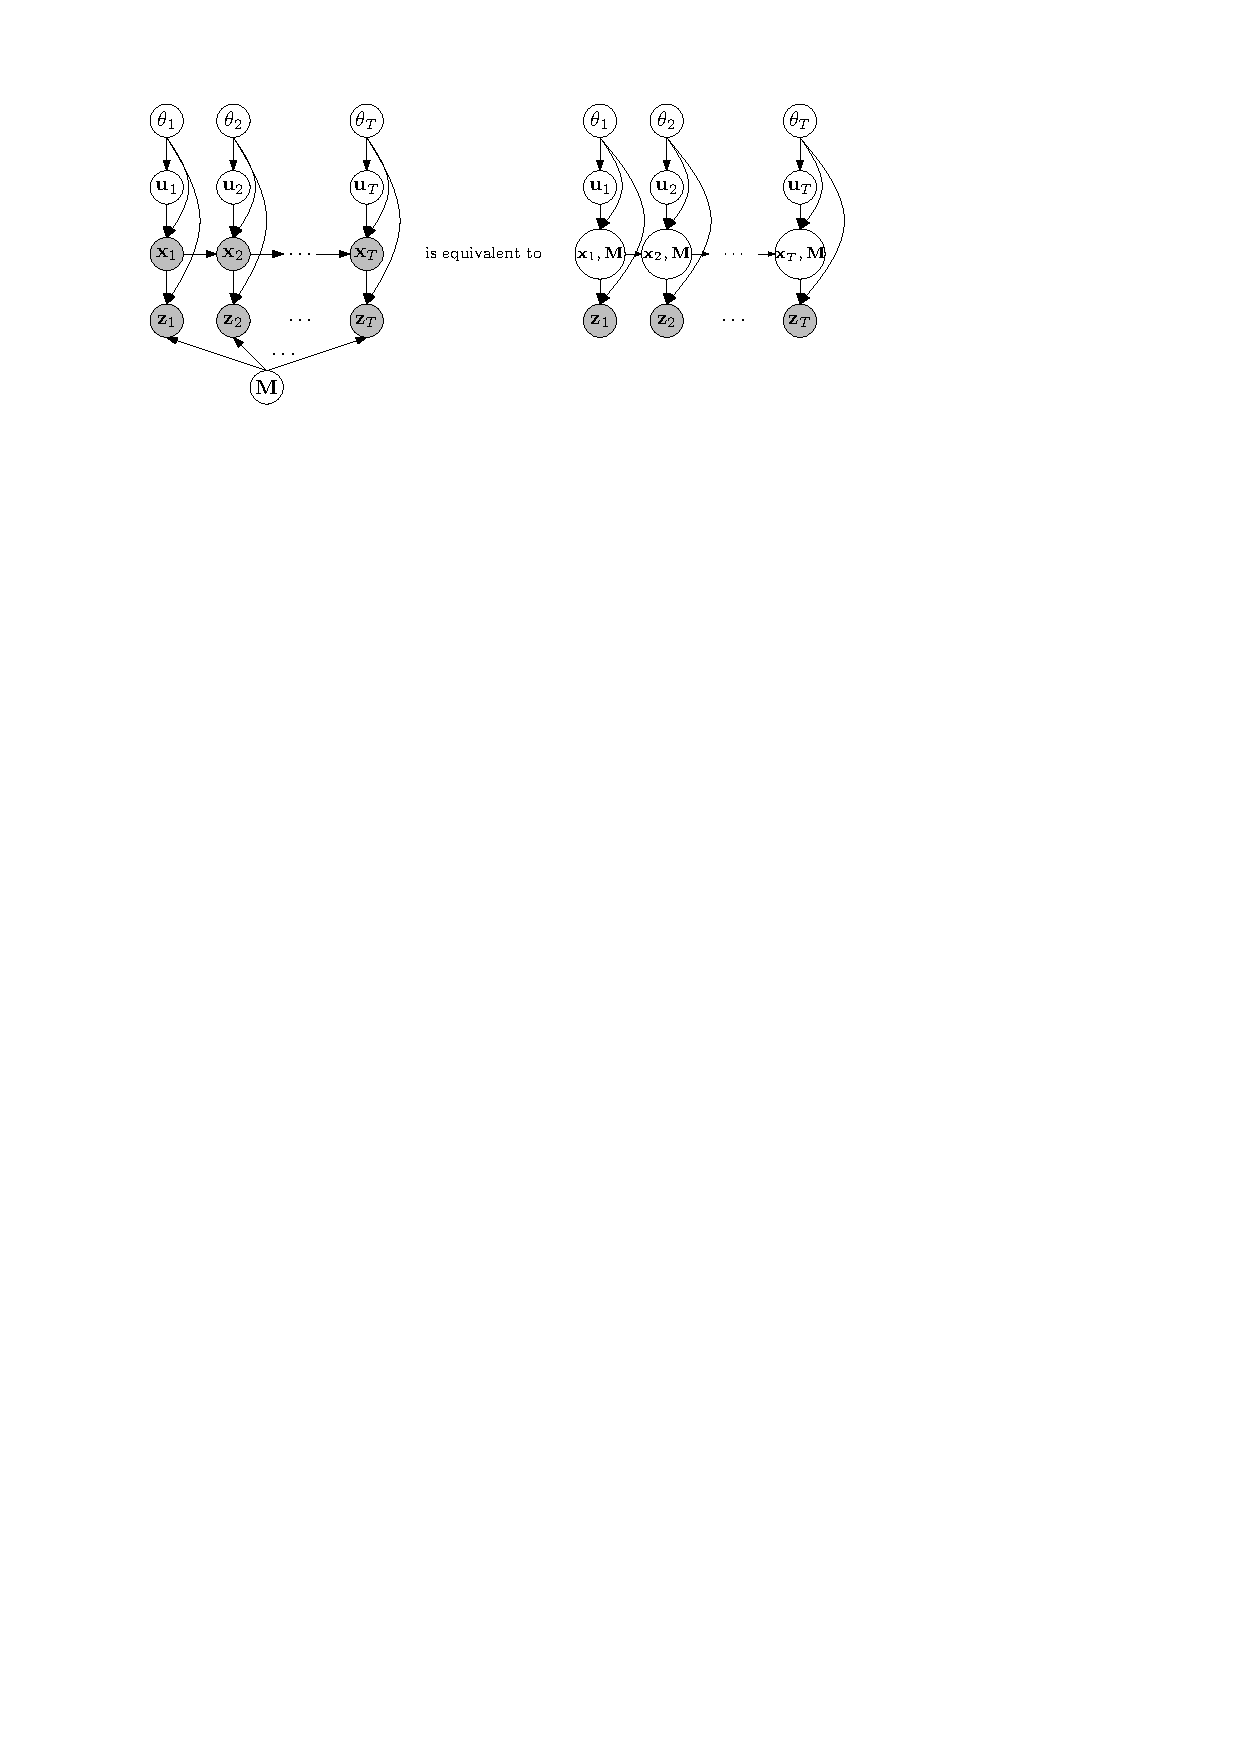
\includegraphics[scale=1]{models/kf/figures/kf-map}
\caption{Probabilistic Graphical Model for the Kalman Filter for Mapping.}
\label{fig:models/kf/figures/kf-map}
\end{figure}

on the left, we shade $\vec x_1, \dotsc, \vec x_T$ and $\vec z_1, \dotsc, \vec z_T$ to signify that they are observed variables. Note that since both the observation and the states are now observed, the directed edges between them are now redundant (but are left there for clarity). On the right, we group the $\vec x$'s and $\vec M$ together. We call these random variables, for $t = 1, \dotsc, T$
\begin{equation}
	\vec x_t^\ast =
		\begin{bmatrix}
			\vec x_t \\
			\vec M
		\end{bmatrix}
\end{equation}
Since these random variables are only ``half-observed'', we don't shade them.

The model can be described, for $t = 1, \dotsc, T$, by the following equations:
\begin{align}
	\vec x_t^\ast 	&= \vec g^\ast(\vec x_{t - 1}^\ast, \vec u_t) + \vec \epsilon_t^\ast \\
	\vec z_t 		&= \vec h^\ast(\vec x_t^\ast, \vec u_t) + \vec \delta_t^\ast
\end{align}
We need to characterise $\vec g^\ast(\vec x^\ast, \vec u)$, $\vec \epsilon_t^\ast$, $\vec h^\ast(\vec x^\ast, \vec u)$, and $\vec \delta_t^\ast$ to describe the EKF algorithm fully.

\subsubsection{The transition model}
The transition model is described by
\begin{align}
	\vec g^\ast(\vec x^\ast_{t - 1}, \vec u_t) = 
		\begin{bmatrix}
			\vec x_t \\
			\vec M
		\end{bmatrix}
\end{align}
and
\begin{align}
	\vec Q_t = 
		\begin{bmatrix}
			\vec 0_{n \times n}		& \vec 0_{n \times Kd} \\
			\vec 0_{Kd \times n}	& \vec Q_{t, M}
		\end{bmatrix}
\end{align}
where $\vec Q_{t, M}$ is the covariance for $\vec M$ at time $t$.

\subsubsection{The observation model}
The observation model is defined for the observation variable is the same as the one in the Localisation case, described in the Subsubsection~\ref{subsubsec:models/kf/localisation/obs}, in Equations~\eqref{eqn:models/kf/localisation/obs} and \eqref{eqn:models/kf/localisation/obs2}. The observation model is then
\begin{align}
	\vec h^\ast(\vec x^\ast_t, \vec u_t) =
									\begin{bmatrix}
										\|\vec m_{c_{t, 1}} - (x_t, y_t)^T\| \\
										\arctan\left((m_{c_{t, 1}, y} - y_t) / (m_{c_{t, 1}, x} - x_t) \right) - \theta_t \\
										\vdots \\
										\|\vec m_{c_{t, \ell}} - (x_t, y_t)^T\| \\
										\arctan\left((m_{c_{t, \ell}, y} - y_t) / (m_{c_{t, \ell}, x} - x_t) \right) - \theta_t \\
										\vdots \\
										\|\vec m_{c_{t, L}} - (x_t, y_t)^T\| \\
										\arctan\left((m_{c_{t, L}, y} - y_t) / (m_{c_{t, L}, x} - x_t) \right) - \theta_t
									\end{bmatrix}
\end{align}
and
\begin{align}
	\vec R_t = \diag(\sigma^2_r, \sigma^2_\phi, \dotsc, \sigma^2_r, \sigma^2_\phi) \in \mathbb R^{2L \times 2L}
\end{align}
Note that the observation model is very similar to the one in the Localisation case, the only differences being grouping of $\vec x, \vec M$ into $\vec x^\ast$.